\section{Tổng quan về các kiến trúc phần mềm}

\begin{flushleft}
  \hspace*{0.8cm}Trong quá trình phát triển ứng dụng di động, kiến trúc phần mềm không chỉ đóng vai trò định hình cấu trúc của mã nguồn mà còn ảnh hưởng trực tiếp đến khả năng mở rộng, bảo trì và hiệu suất vận hành của toàn bộ hệ thống. Việc lựa chọn mô hình kiến trúc phù hợp với tính chất của ứng dụng và nền tảng triển khai sẽ giúp các lập trình viên tối ưu quy trình phát triển, đồng thời nâng cao tính linh hoạt và khả năng tái sử dụng của mã nguồn. Trong chương này, chúng ta sẽ lần lượt khảo sát một số mẫu kiến trúc phần mềm phổ biến như mô hình phân lớp (Layers), kiến trúc MVC – thường gặp trên iOS, kiến trúc MVVM – được ưa chuộng trong Android hiện đại, và mô hình giao tiếp Client–Server. Qua đó, chương này nhằm mục tiêu cung cấp cái nhìn toàn diện về cách các kiến trúc phần mềm góp phần vào việc xây dựng những ứng dụng di động ổn định, dễ mở rộng và đáp ứng tốt nhu cầu người dùng.
\end{flushleft}

% 3.1
\subsection{Mẫu kiến trúc Layers}
\renewcommand{\labelitemi}{--}    
\begin{flushleft}
    \hspace*{0.8cm}Một trong những mẫu kiến trúc nền tảng và phổ biến nhất trong phát triển phần mềm là kiến trúc phân lớp (Layers). Mô hình này được áp dụng rộng rãi trên cả hai nền tảng iOS và Android do khả năng tổ chức mã nguồn theo hướng tách biệt rõ ràng từng chức năng. Trong kiến trúc Layers, ứng dụng được chia thành ba lớp chính: lớp giao diện (Presentation Layer), lớp xử lý nghiệp vụ (Business Logic Layer), và lớp dữ liệu (Data Layer). Mỗi lớp đảm nhiệm một vai trò riêng biệt, giúp cấu trúc hệ thống trở nên rõ ràng, dễ hiểu và dễ kiểm soát.
\end{flushleft}

% https://viquynh.wordpress.com/2018/02/05/mo-hinh-mvc2-code-demo-jsp-servlet-javabe/
\begin{figure}[H]
    \centering
    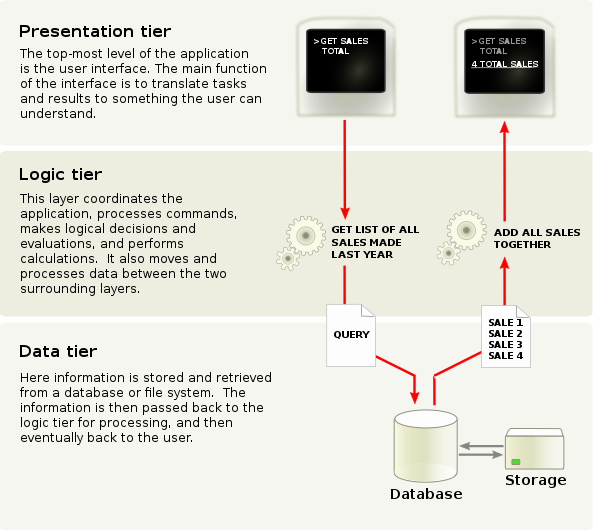
\includegraphics[width=0.75\textwidth]{images/layer.png}
    \caption{Mô hình kiến trúc 3 tầng (3-tiers) \cite{viquynhMVC2}.}
    \label{fig:fig11}
  \end{figure}
    
    \begin{flushleft}
        \hspace*{0.8cm}Cụ thể, lớp Presentation đóng vai trò là điểm tương tác giữa người dùng và hệ thống, chịu trách nhiệm hiển thị thông tin và thu nhận thao tác từ phía người dùng. Lớp Business Logic là nơi xử lý toàn bộ logic nghiệp vụ, từ kiểm tra dữ liệu nhập vào đến các phép tính, xử lý trạng thái và ra quyết định. Cuối cùng, lớp Data đảm nhiệm vai trò giao tiếp với nguồn dữ liệu – có thể là cơ sở dữ liệu cục bộ hoặc server từ xa – và thực hiện các thao tác đọc, ghi hoặc đồng bộ hóa.
    
    \end{flushleft}
    
    \begin{flushleft}
        \hspace*{0.8cm}Ưu điểm nổi bật của mô hình Layers là tính phân tách trách nhiệm (separation of concerns). Mỗi lớp chỉ đảm nhiệm một nhóm chức năng chuyên biệt, nên khi có thay đổi hoặc lỗi phát sinh ở một lớp, lập trình viên có thể xử lý mà không ảnh hưởng đến các lớp còn lại. Điều này đặc biệt quan trọng trong các dự án lớn hoặc khi có nhiều lập trình viên cùng tham gia. Ngoài ra, việc kiểm thử (testing) cũng trở nên dễ dàng hơn nhờ tính độc lập giữa các lớp. Tuy nhiên, mô hình này cũng có thể dẫn đến sự phụ thuộc theo chiều dọc giữa các lớp nếu không được thiết kế đúng cách, và đôi khi làm tăng số lượng lớp và khối lượng mã khi ứng dụng phát triển phức tạp hơn.
    \end{flushleft}
    
    \begin{flushleft}
        \hspace*{0.8cm}Nhìn chung, kiến trúc phân lớp đóng vai trò như một mô hình nền tảng, thích hợp với nhiều loại ứng dụng khác nhau. Nhờ khả năng tổ chức tốt và dễ mở rộng, mô hình này thường được sử dụng làm cơ sở cho các kiến trúc phức tạp hơn như MVC hay MVVM, đóng góp vào việc xây dựng phần mềm có cấu trúc bền vững và hiệu quả.
    \end{flushleft}

% 3.2
\subsection{Mẫu kiến trúc MVC}
\renewcommand{\labelitemi}{--}    
    \begin{flushleft}
        \hspace*{0.8cm}Trong số các mô hình kiến trúc phần mềm được áp dụng trên nền tảng iOS, Model–View–Controller (MVC) là một trong những mô hình lâu đời và phổ biến nhất. MVC chia ứng dụng thành ba thành phần chính, từ đó giúp lập trình viên dễ dàng tổ chức mã nguồn và phân tách nhiệm vụ của từng bộ phận trong quá trình phát triển. Trong đó, thành phần Model đảm nhiệm vai trò quản lý dữ liệu và xử lý các quy tắc nghiệp vụ, đóng vai trò như “bộ não” của ứng dụng. Tiếp theo, thành phần View chịu trách nhiệm hiển thị thông tin tới người dùng, phản ánh đúng trạng thái hiện tại của dữ liệu từ Model. Cuối cùng, thành phần Controller đóng vai trò trung gian, cầu nối giữa View và Model, đảm nhận việc xử lý các sự kiện tương tác của người dùng, đồng thời cập nhật lại giao diện khi dữ liệu thay đổi.
    \end{flushleft}

    % https://daynhauhoc.com/t/loi-load-du-lieu-len-jsp/109965/10
\begin{figure}[H]
    \centering
    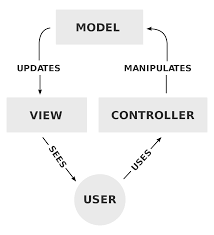
\includegraphics[width=0.5\textwidth]{images/mvc.png}
    \caption{Mô hình kiến trúc MVC \cite{daynhauhocMVC}.}
    \label{fig:fig12}
  \end{figure}

    \begin{flushleft}
      \hspace*{0.8cm}Với cấu trúc như vậy, mô hình MVC mang đến cho lập trình viên iOS một cách tiếp cận đơn giản, dễ hiểu, phù hợp với những người mới bắt đầu tiếp cận lập trình giao diện người dùng. Tuy nhiên, trong thực tế triển khai, một vấn đề lớn phát sinh là hiện tượng “Massive View Controller” \cite{massive_vc}, khi Controller bị quá tải do chứa cả logic giao diện lẫn logic nghiệp vụ. Điều này dẫn đến mã nguồn trở nên khó bảo trì, khó kiểm thử và dễ phát sinh lỗi khi mở rộng chức năng. Chính vì thế, ngày càng nhiều lập trình viên iOS hiện đại chuyển sang các mô hình khác như MVVM hoặc VIPER để giảm thiểu sự phụ thuộc và tách biệt rõ ràng các thành phần chức năng hơn. Nhìn chung, mặc dù MVC vẫn giữ được tính phổ biến nhất định, đặc biệt trong các ứng dụng đơn giản, nhưng nó không còn là lựa chọn tối ưu trong các dự án phức tạp hoặc quy mô lớn.
    \end{flushleft}

% 3.3
\subsection{Mô hình kiến trúc MVVM}
\renewcommand{\labelitemi}{--}    
    \begin{flushleft}
        \hspace*{0.8cm}Trên nền tảng Android, mô hình kiến trúc Model–View–ViewModel (MVVM) ngày càng trở nên phổ biến nhờ khả năng tương thích cao với các thư viện hỗ trợ hiện đại như LiveData, ViewModel, và Data Binding. MVVM được thiết kế để tách biệt rõ ràng giữa giao diện người dùng và logic nghiệp vụ, đồng thời hỗ trợ tốt cho việc phát triển theo hướng phản ứng (reactive programming). Trong mô hình này, Model tiếp tục đảm nhiệm vai trò quản lý dữ liệu và xử lý các quy tắc nghiệp vụ, tương tự như trong mô hình MVC. View, tức giao diện người dùng, có nhiệm vụ hiển thị dữ liệu và nhận tương tác từ người dùng, tuy nhiên, thay vì xử lý trực tiếp các thao tác đó, View sẽ truyền tín hiệu cho ViewModel để xử lý.
    \end{flushleft}

    % https://teky.edu.vn/blog/lap-trinh-web-mvc/
\begin{figure}[H]
    \centering
    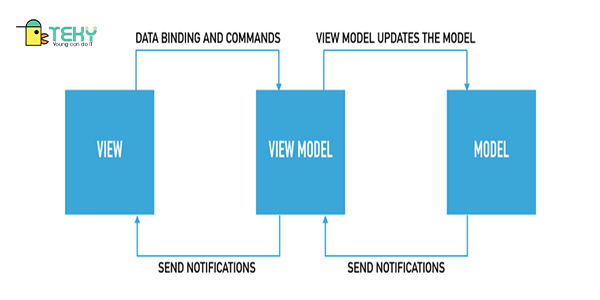
\includegraphics[width=0.67\textwidth]{images/mvvm.jpg}
    \caption{Mô hình kiến trúc MVVM \cite{tekyMVVM}}
    \label{fig:fig13}
  \end{figure}

    \begin{flushleft}
      \hspace*{0.8cm}Thành phần cốt lõi giúp MVVM trở nên nổi bật chính là ViewModel – lớp trung gian giữa View và Model. ViewModel không chứa tham chiếu trực tiếp tới View, mà hoạt động dựa trên cơ chế observer pattern, cho phép dữ liệu được quan sát và cập nhật tự động từ ViewModel lên View mỗi khi có thay đổi. Nhờ đó, View trở nên “mỏng” hơn vì chỉ tập trung vào hiển thị, còn toàn bộ logic xử lý sự kiện, tính toán hoặc tương tác với dữ liệu được chuyển giao sang ViewModel. Cách tiếp cận này không những giúp giảm sự ràng buộc giữa các lớp, mà còn tăng khả năng tái sử dụng, kiểm thử tự động và phát triển song song giữa các thành viên trong nhóm \cite{testability_mvvm}.
    \end{flushleft}

    \begin{flushleft}
        \hspace*{0.8cm}Tóm lại, MVVM phù hợp với xu hướng phát triển ứng dụng hiện đại trên Android khi đặt trọng tâm vào tính phân tách, phản ứng và mở rộng. So với các mô hình truyền thống như MVC, MVVM mang lại kiến trúc rõ ràng hơn và giúp lập trình viên kiểm soát ứng dụng hiệu quả trong cả giai đoạn phát triển lẫn bảo trì.
    \end{flushleft}

% 3.4
\subsection{Hỗ trợ mô hình Client – Server}
\renewcommand{\labelitemi}{--}    
    \begin{flushleft}
        \hspace*{0.8cm}Trong quá trình xây dựng ứng dụng di động hiện đại, mô hình Client–Server luôn đóng vai trò then chốt trong việc hỗ trợ các chức năng có kết nối mạng. Cả hai nền tảng iOS và Android đều cung cấp đầy đủ công cụ để triển khai mô hình này một cách hiệu quả. Trong mô hình Client–Server, ứng dụng di động đóng vai trò như Client, có nhiệm vụ gửi các yêu cầu (request) tới một máy chủ từ xa (Server) thông qua các giao thức HTTP với các phương thức như GET, POST, PUT, DELET. Sau khi tiếp nhận yêu cầu, Server sẽ xử lý thông tin, truy xuất cơ sở dữ liệu và trả về kết quả dưới dạng JSON hoặc XML để Client hiển thị hoặc xử lý tiếp theo.
    \end{flushleft}

    % https://codelearn.io/sharing/tim-hieu-ve-mo-hinh-client-server
\begin{figure}[H]
    \centering
    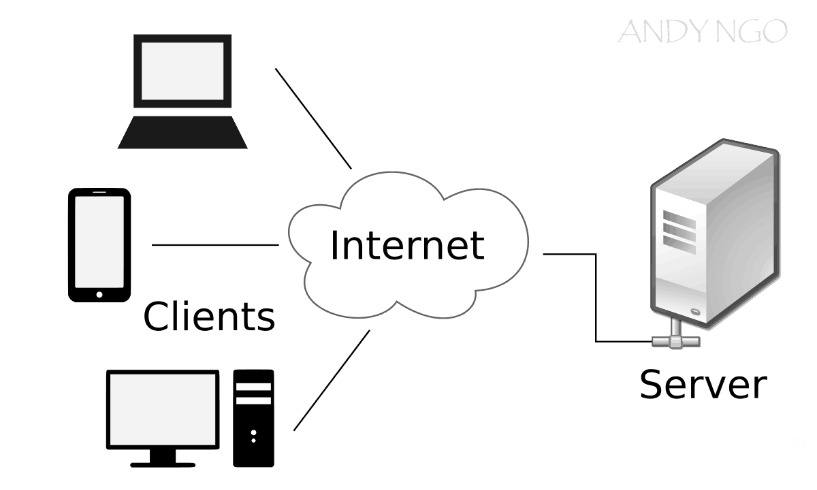
\includegraphics[width=0.75\textwidth]{images/client-server.jpg}
    \caption{Mô hình Client – Server \cite{codelearnClientServer}.}
    \label{fig:fig14}
  \end{figure}

    \begin{flushleft}
      \hspace*{0.8cm}Để hỗ trợ tốt cho mô hình này, các hệ điều hành di động đều cung cấp nhiều thư viện mạnh mẽ. Trên iOS, lập trình viên có thể sử dụng URLSession như một công cụ tiêu chuẩn từ Apple hoặc tích hợp thư viện bên thứ ba như Alamofire để đơn giản hóa các tác vụ mạng. Tương tự, Android cung cấp các thư viện Retrofit và OkHttp giúp việc gửi yêu cầu và xử lý phản hồi trở nên nhanh chóng, dễ mở rộng và dễ kiểm thử. Thông qua mô hình Client–Server, ứng dụng di động có thể hoạt động nhẹ nhàng hơn vì dữ liệu và logic nặng được xử lý ở phía máy chủ. Ngoài ra, tính năng đồng bộ dữ liệu và cập nhật thời gian thực giữa nhiều thiết bị người dùng cũng được hiện thực hóa dễ dàng thông qua mô hình này. Điều này cho thấy Client–Server không chỉ là một mô hình kết nối, mà còn là nền tảng cốt lõi giúp ứng dụng thích ứng linh hoạt trong môi trường đa thiết bị và thay đổi liên tục ngày nay \cite{scalable_mobile_arch}.
    \end{flushleft}

% 3.5
\subsection{Đánh giá tổng quan}
\renewcommand{\labelitemi}{--}    
    \begin{flushleft}
        \hspace*{0.8cm}Dưới góc nhìn tổng quan, các mô hình kiến trúc phần mềm như MVC, MVVM và Client–Server đều mang đến những giá trị thiết thực trong việc phát triển ứng dụng di động. Tuy nhiên, mỗi nền tảng lại có sự ưu tiên khác nhau trong cách tiếp cận và tổ chức mã nguồn. Đối với nền tảng iOS, mô hình MVC từng được xem là tiêu chuẩn “vàng” nhờ vào sự đơn giản và dễ học. Thế nhưng, hạn chế lớn nhất của MVC – đó là hiện tượng “Massive View Controller” – đã khiến nhiều lập trình viên tìm đến các mô hình thay thế để có được cấu trúc tách biệt và linh hoạt hơn \cite{massive_view_controller}.
    \end{flushleft}

    \begin{flushleft}
        \hspace*{0.8cm}Trong khi đó, Android hiện đại hóa cách tổ chức ứng dụng thông qua mô hình MVVM, tận dụng sức mạnh từ các thành phần như LiveData, ViewModel và Data Binding. Nhờ vậy, lập trình viên có thể giảm mạnh sự phụ thuộc giữa giao diện và logic nghiệp vụ, đồng thời tối ưu khả năng tái sử dụng và kiểm thử mã nguồn. Ngoài ra, cả iOS và Android đều đồng thuận trong việc triển khai mô hình Client–Server nhằm tăng khả năng mở rộng, giảm tải cho thiết bị người dùng và hỗ trợ ứng dụng hoạt động ổn định trong môi trường mạng. Việc nắm rõ đặc điểm, ưu điểm cũng như nhược điểm của từng mô hình kiến trúc sẽ giúp lập trình viên không chỉ lựa chọn đúng giải pháp cho từng dự án cụ thể, mà còn góp phần nâng cao hiệu quả phát triển, khả năng bảo trì và mở rộng sản phẩm trong dài hạn.
    \end{flushleft}
